\documentclass[aspectratio=169,10pt]{beamer}
% ------------------------------------------------------------------
% Spin transport project: source-based introductory Beamer deck.
% Reference: project state of 15 October 2026, xxz_open_edges_revised(5).m
% (H_ZZ, H_XY: chapters 10-11; dynamics engine: chapters 5-9, homogeneous
% xxzH only), XXZ_verification_report.md, edge_map_implementation_guide.md.
% XXZ_v3_current_state.md is NOT used: it does not describe the current file.
% Revised 15 Oct 2026: every claim re-derived; the numbers on the appendix
% slide come from independent small-L dense ED in Wolfram Language 15.0.1,
% not from production runs of the notebook.
% ------------------------------------------------------------------
\usepackage[T1]{fontenc}
\usepackage{lmodern}
\usepackage{amsmath,amssymb,mathtools,bm}
\usepackage{booktabs,array}
\usepackage{tikz}
\usetikzlibrary{arrows.meta,positioning,calc,decorations.pathreplacing}
\usepackage{xcolor}
\definecolor{ink}{HTML}{182B40}
\definecolor{muted}{HTML}{5D7185}
\definecolor{sea}{HTML}{007C8A}
\definecolor{royal}{HTML}{4168A2}
\definecolor{amber}{HTML}{B06B21}
\definecolor{pale}{HTML}{EFF4F7}
\definecolor{linegray}{HTML}{D9E3E9}
\definecolor{cardgray}{HTML}{F7F9FB}
\setbeamercolor{normal text}{fg=ink,bg=white}
\setbeamercolor{frametitle}{fg=ink,bg=white}
\setbeamercolor{structure}{fg=sea}
\setbeamercolor{itemize item}{fg=sea}
\setbeamercolor{itemize subitem}{fg=sea}
\setbeamercolor{block title}{fg=white,bg=ink}
\setbeamercolor{block body}{fg=ink,bg=pale}
\setbeamertemplate{navigation symbols}{}
\setbeamertemplate{itemize item}{\raisebox{.2ex}{\tiny$\blacktriangleright$}}
\setbeamertemplate{frametitle}{%
  \vspace{0.13cm}\hspace{0.45cm}\insertframetitle\par%
  \vspace{0.09cm}\hspace{0.45cm}{\color{sea}\rule{14.75cm}{0.6pt}}\vspace{0.07cm}%
}
\setbeamertemplate{footline}{%
  \leavevmode\hbox{%
    \begin{beamercolorbox}[wd=.83\paperwidth,ht=2.8ex,dp=1.15ex,leftskip=.47cm]{normal text}%
      {\color{muted}\scriptsize Spin transport \quad/\quad XXZ boundary probes \quad/\quad physical framework (15 Oct 2026)}%
    \end{beamercolorbox}%
    \begin{beamercolorbox}[wd=.17\paperwidth,ht=2.8ex,dp=1.15ex,rightskip=.48cm plus1fil]{normal text}%
      {\color{sea}\scriptsize\hfill\insertframenumber\,/\,\inserttotalframenumber}%
    \end{beamercolorbox}}%
}
\setlength{\parskip}{4pt}
\setbeamersize{text margin left=.56cm,text margin right=.56cm}
\newcommand{\Sz}[1]{S_{#1}^{z}}
\newcommand{\Tr}{\operatorname{Tr}}
\newcommand{\ket}[1]{\lvert #1\rangle}
\newcommand{\bra}[1]{\langle #1\rvert}
\newcommand{\vN}[1]{S(#1)}
\newcommand{\rhoAB}{\rho_{AB}}
\newcommand{\Hb}{H_{\mathrm{bulk}}}
\newcommand{\HH}{H_{\mathrm{hom}}}
\newcommand{\Hzz}{H_{\mathrm{ZZ}}}
\newcommand{\Hxy}{H_{\mathrm{XY}}}
\newcommand{\sechead}[1]{{\color{sea}\bfseries #1}\par\vspace{1mm}}
\newcommand{\noteinline}[1]{{\color{muted}\footnotesize #1}}
\newcommand{\mathkey}[1]{{\color{sea}\textsf{#1}}}
\newcommand{\smallrule}{\par\vspace{1mm}\noindent{\color{linegray}\rule{\linewidth}{0.6pt}}\par\vspace{1mm}}
\title{Boundary spin probes in an open XXZ chain}
\subtitle{Symmetry constraints, conditional dynamics, and the edge quantum channel}
\author{Spin transport project}
\date{October 2026 \;|\; Physical framework}

\begin{document}
\begin{frame}[plain]
  \vspace{1.05cm}
  {\color{sea}\large SPIN TRANSPORT \; / \; PHYSICAL SETUP}\par\vspace{.42cm}
  {\color{ink}\bfseries\fontsize{25}{29}\selectfont Boundary spin probes\par in an open XXZ chain}\par\vspace{.30cm}
  {\color{muted}\large Boundary interactions \;\textbullet\; Conserved charges \;\textbullet\; Reduced dynamics}\par
  \vfill
  {\color{muted}\small Exact constraints on two-edge reduced dynamics and quantum channels}\par
  {\color{sea}\small 15 October 2026}
\end{frame}

\begin{frame}{Research question: what information survives at the edges?}
\begin{columns}[T,onlytextwidth]
\column{.54\textwidth}
\sechead{A local window onto a many-body system}
The full chain evolves unitarily, but only the two end spins are observed. We ask which features of the interacting interior constrain or remain visible in their joint reduced state.
\begin{itemize}\setlength\itemsep{5pt}
  \item What can the ends exchange with the bulk?
  \item Which coherences and correlations can develop?
  \item What structural restrictions does symmetry impose on the reduced map?
\end{itemize}
\column{.44\textwidth}
\begin{block}{Central object}
\[\rho_{AB}(t)=\Tr_{E}\!\left[U(t)\rho_{ABE}(0)U(t)^\dagger\right]\]
\smallskip
For a \emph{fixed, uncorrelated} bulk preparation \(\omega_E\),
\[\rho_{AB}(t)=\Lambda_t[\rho_{AB}(0)].\]
\end{block}
\end{columns}
\smallskip
\noteinline{The reduced state is an observable for any full-chain initial condition; a CPTP map on arbitrary edge inputs requires a fixed environment preparation.}
\end{frame}

\begin{frame}{Geometry: two end spins and an XXZ interior}
  \begin{center}
  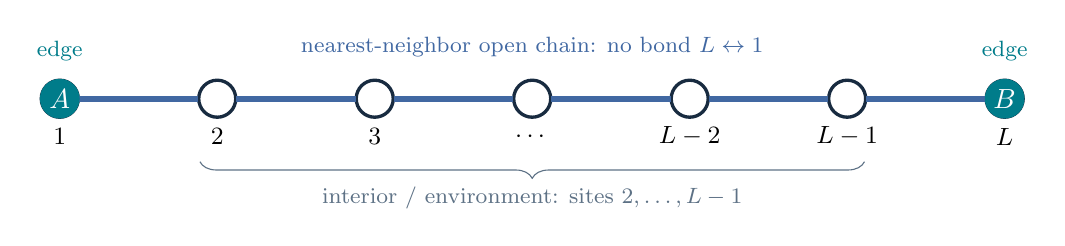
\begin{tikzpicture}[x=1cm,y=1cm]
    \foreach \x/\lab in {0/1,2/2,4/3,6/\cdots,8/{L-2},10/{L-1},12/L}{
      \filldraw[fill=white,draw=ink,line width=1.2pt] (\x,0) circle (0.235);
      \node[font=\small] at (\x,-.48) {$\lab$};
    }
    \foreach \x in {0,2,4,6,8,10}{\draw[line width=2.1pt,color=royal] (\x+.24,0)--(\x+1.76,0);}
    \filldraw[fill=sea,draw=sea] (0,0) circle (.245);
    \filldraw[fill=sea,draw=sea] (12,0) circle (.245);
    \node[white,font=\bfseries] at (0,0) {$A$};
    \node[white,font=\bfseries] at (12,0) {$B$};
    \node[font=\footnotesize,color=sea] at (0,0.61) {edge};
    \node[font=\footnotesize,color=sea] at (12,0.61) {edge};
    \draw[decorate,decoration={brace,amplitude=6pt,mirror},color=muted] (1.78,-.80)--(10.22,-.80);
    \node[color=muted,font=\footnotesize] at (6,-1.26) {interior / environment: sites $2,\ldots,L-1$};
    \node[color=royal,font=\footnotesize] at (6,.66) {nearest-neighbor open chain: no bond $L\leftrightarrow1$};
  \end{tikzpicture}
  \end{center}
  \vspace{.20cm}
  \begin{columns}[T,onlytextwidth]
    \column{.48\textwidth}
      \sechead{Hilbert space and convention}
      $\mathcal H=(\mathbb C^2)^{\otimes L}$, \quad $S_i^\alpha=\sigma_i^\alpha/2$, \quad $\hbar=1$.
      \par Computational basis: bit $0=\uparrow$, bit $1=\downarrow$.
    \column{.48\textwidth}
      \sechead{The subsystem of interest}
      $\mathcal H_{AB}=\mathbb C^2\otimes\mathbb C^2$; basis $\{\ket{00},\ket{01},\ket{10},\ket{11}\}$.
      \par $\rhoAB(t)=\Tr_{2,\ldots,L-1}\{\rho(t)\}$.
  \end{columns}
\end{frame}

\begin{frame}{The model: an interacting interior, two different edge bonds}
\sechead{Common XXZ interior, open boundaries}
\[
H_E=J\sum_{j=2}^{L-2}\!\left(S_j^x S_{j+1}^x+S_j^yS_{j+1}^y+\Delta S_j^zS_{j+1}^z\right),
\qquad S^\alpha=\frac{\sigma^\alpha}{2}.
\]
\vspace{.04cm}
\begin{columns}[T,onlytextwidth]
\column{.49\textwidth}
\sechead{Longitudinal boundary coupling}
\[
\boxed{H_{\rm ZZ}=H_E+g(S_1^zS_2^z+S_{L-1}^zS_L^z)}
\]
\smallskip
No boundary spin flips.
\column{.49\textwidth}
\sechead{Transverse exchange coupling}
\[
\boxed{H_{\rm XY}=H_E+g\!\!\!\sum_{(i,j)\in\partial}\!\!\!(S_i^xS_j^x+S_i^yS_j^y)}
\]
\smallskip
\(\partial=\{(1,2),(L-1,L)\}\): flip-flop transport.
\end{columns}
\smallskip
\par\vspace{.10cm}
\noteinline{The original end bonds are replaced. The boundary coefficient \(g\) has energy units; longitudinal fields preserve the ZZ edge-charge conservation.}
\end{frame}


\begin{frame}{Symmetries: magnetization, edge charges, reflection, and spin flip}
\begin{columns}[T,onlytextwidth]
\column{.45\textwidth}
\sechead{Magnetizations and edge charges}
\(M=\sum_{j=1}^{L}S_j^z\), \(M_E=\sum_{j=2}^{L-1}S_j^z\), with eigenvalues \(m\), \(m_E\).
\par\vspace{.12cm}
\(s,t=\pm\tfrac12\): eigenvalues of \(S_1^z\), \(S_L^z\) (\(+\tfrac12\equiv\uparrow\), bit 0); \(\ket{s,t}\equiv\ket{s}_1\ket{t}_L\).
\column{.52\textwidth}
\sechead{Reflection R and global spin flip F}
\(R\ket{\sigma_1\sigma_2\cdots\sigma_L}=\ket{\sigma_L\cdots\sigma_2\sigma_1}\),\quad \(F=\prod_{j=1}^{L}\sigma_j^x\).
\par\vspace{.08cm}
\(R^2=F^2=1\), \([R,F]=0\), \(RMR=M\), \(FMF=-M\).
\par\vspace{.08cm}
\(R=\mathrm{SWAP}_{AB}\otimes R_E\), \(F=(\sigma^x\!\otimes\sigma^x)_{AB}\otimes F_E\): \(R_E\) reverses sites \(2,\ldots,L-1\), \(F_E=\prod_{j=2}^{L-1}\sigma_j^x\).
\end{columns}
\vspace{.15cm}
\begin{block}{When they apply}
Both commute with \(H_{\rm ZZ}\) and \(H_{\rm XY}\) when the two end couplings are equal and all \(z\) fields vanish. On ZZ labels: \(R\colon(s,t,m_E)\mapsto(t,s,m_E)\), \(F\colon(s,t,m_E)\mapsto(-s,-t,-m_E)\).
\end{block}
\vspace{.05cm}
\noteinline{Since \(F\) reverses \(M\), it is a quantum number only at \(m=0\). In fixed-\((s,t)\) blocks, \(R\) is a label only for \(s=t\), and \(RF\) only for \(s=-t\), \(m_E=0\).}
\end{frame}


\begin{frame}{Two boundary regimes, two kinds of reduced dynamics}
\begin{columns}[T,onlytextwidth]
\column{.49\textwidth}
\sechead{I. ZZ: conditional many-body evolution}
\begin{itemize}\setlength\itemsep{7pt}
\item Each edge \(S^z\) is \emph{separately} conserved.
\item Edges act as quantum controls for the bulk's boundary fields.
\item Joint edge populations are constants; coherence can be lost or recovered.
\item The reduced map is exactly a joint-basis dephasing channel.
\end{itemize}
\column{.49\textwidth}
\sechead{II. XY: excitation exchange}
\begin{itemize}\setlength\itemsep{7pt}
\item Individual edge \(S^z\) values need not be conserved.
\item Of the \(U(1)\) charges only total \(M\) survives (\(R\), \(F\) remain).
\item Both edge populations and coherences can evolve.
\item Symmetry constrains the map, but does not force dephasing.
\end{itemize}
\end{columns}
\vspace{.24cm}
\noteinline{This is a comparison of \emph{boundary coupling mechanisms}; the interior anisotropy \(\Delta\) is an independent physical control.}
\end{frame}


\begin{frame}{Which exact symmetries matter for the edges?}
\begin{columns}[T,onlytextwidth]
\column{.51\textwidth}
\sechead{ZZ-only boundary bonds}
\[
[H_{\rm ZZ},S_1^z]=[H_{\rm ZZ},S_L^z]=0.
\]
\[[H_{\rm ZZ},M_E]=0.\]
\smallskip
Independent sector labels: \((s,t,m_E)\).
\par
\textbf{Not implied:} \([H_{\rm ZZ},S_1^zS_2^z]=0\). The boundary coupling is dynamically consequential.
\column{.47\textwidth}
\sechead{XY-only boundary bonds}
\[
[H_{\rm XY},M]=0,
\]
\[
[H_{\rm XY},S_{1,L}^z]\neq0\quad(g\ne0).
\]
\smallskip
For equal end couplings and zero fields, \(R\) and \(F\) commute with both \(H_{\rm XY}\) and \(H_{\rm ZZ}\).
\end{columns}
\smallrule
\noteinline{In the ZZ model \(R\) and \(F\) move \((s,t,m_E)\) between blocks, so they are not extra quantum numbers within every fixed-charge block.}
\end{frame}


\begin{frame}{ZZ regime: exact controlled-Hamiltonian structure}
Let \(s,t=\pm\tfrac12\) be the eigenvalues of \(S_1^z\) and \(S_L^z\) (\(+\tfrac12\equiv\uparrow\), bit 0), \(a=(s,t)\), and \(P_a=\ket{a}\!\bra{a}\) the projector onto \(\ket{s}_1\ket{t}_L\). Then
\[
\boxed{H_{\rm ZZ}=\sum_a P_a\otimes K_a,\qquad
K_a\equiv K_{s,t}=H_E+g(sS_2^z+tS_{L-1}^z),\qquad a=(s,t).}
\]
\vspace{-.11cm}
\[
\boxed{U(t)=\sum_a P_a\otimes U_a(t),\qquad U_a(t)=e^{-iK_at}.}
\]
\begin{columns}[T,onlytextwidth]
\column{.51\textwidth}
\sechead{Physical meaning}
The edges never flip. The interior feels them \emph{only} through two longitudinal fields: \(gs\) on site 2 and \(gt\) on site \(L-1\). The bulk still propagates and interacts.
\column{.46\textwidth}
\sechead{Why this is useful}
A single many-body evolution is replaced by four conditional bulk evolutions. Their mutual overlaps determine the reduced edge channel exactly.
\end{columns}
\smallskip
\noteinline{Longitudinal bulk/edge fields only modify \(K_a\) (edge fields add constants); the decomposition survives.}
\end{frame}


\begin{frame}{A zero-entanglement eigenbasis is guaranteed, but not unique}
Since each \(K_a\) is Hermitian, it has a complete eigenbasis \(\{\ket{\phi_{a,n}}\}\). Hence
\[
H_{\rm ZZ}\bigl(\ket a\otimes\ket{\phi_{a,n}}\bigr)
=E_{a,n}\bigl(\ket a\otimes\ket{\phi_{a,n}}\bigr).
\]
\[
\boxed{S_{AB|E}\!\left(\ket a\otimes\ket{\phi_{a,n}}\right)=0
\quad \text{for a complete energy eigenbasis}.}
\]
\begin{columns}[T,onlytextwidth]
\column{.49\textwidth}
\sechead{What this establishes}
Zero edge-bulk eigenstate entropy in fixed-\((s,t)\) sectors is exact, independent of bulk integrability, \(g\), and internal bulk entanglement.
\column{.49\textwidth}
\sechead{Necessary qualification}
At zero fields this is unavoidable: \(R\) and \(F\) map each edge sector onto a different one, so \emph{every} level has an exact partner in another edge sector, for every \(g\). The \(F\)-symmetric combinations have \(S_{AB|E}=\ln2\).
\end{columns}
\smallskip
\noteinline{The entropy is basis invariant for a fixed state; degenerate-sector superpositions are different states. The notebook's ZZ eigenbasis is the \((s_A,s_B)\)-resolved choice, so its \(S_{AB|E}=0\) is a property of that choice.}
\end{frame}


\begin{frame}{ZZ dynamics: coherent edges record conditional bulk histories}
For an initially pure product state, \(\ket{\Psi(0)}=\sum_a c_a\ket a\otimes\ket{\phi_0}\),
\[
\ket{\Psi(t)}=\sum_a c_a\ket a\otimes U_a(t)\ket{\phi_0}.
\]
Taking the partial trace gives the \emph{exact} reduced edge matrix,
\[
\boxed{[\rho_{AB}(t)]_{ab}=c_ac_b^*\,\gamma_{ab}(t),\qquad
\gamma_{ab}(t)=\bra{\phi_0}U_b^\dagger(t)U_a(t)\ket{\phi_0}.}
\]
\begin{columns}[T,onlytextwidth]
\column{.49\textwidth}
\sechead{Populations cannot move}
\(\rho_{aa}(t)=|c_a|^2\): every joint computational-basis population is fixed.
\column{.49\textwidth}
\sechead{Coherences are nontrivial}
\(\rho_{ab}(t)\) probes distinguishability of two bulk trajectories under \(K_a\) and \(K_b\).
\end{columns}
\smallskip
\noteinline{For a single occupied edge charge \(a\), the state remains a product across \(AB|E\) at all times, for \emph{any} pure bulk input.}
\end{frame}


\begin{frame}{The exact ZZ dynamical map is a correlated dephasing channel}
Assume the \emph{same fixed} bath state \(\omega_E\) for every edge input, with \(\rho_{ABE}(0)=\rho_{AB}(0)\otimes\omega_E\). Then
\[
\boxed{[\Lambda_t(\rho_{AB})]_{ab}
=\Gamma_{ab}(t)[\rho_{AB}]_{ab},\quad
\Gamma_{ab}(t)=\Tr_E[U_a(t)\omega_E U_b^\dagger(t)].}
\]
\begin{columns}[T,onlytextwidth]
\column{.49\textwidth}
\sechead{Exact channel properties}
\begin{itemize}\setlength\itemsep{3pt}
\item \(\Gamma_{aa}(t)=1\) \(\Rightarrow\) all populations fixed.
\item \(\Gamma(t)\succeq0\) \(\Rightarrow\) the Schur-product map is CPTP.
\item It is unital and commutes with independent edge \(z\)-rotations.
\end{itemize}
\column{.49\textwidth}
\sechead{Crucial distinction}
\(\Lambda_t\) is \emph{not generally} \(\Lambda_t^A\otimes\Lambda_t^B\). Both end spins interrogate the same interior, giving potentially correlated coherence decay and phase shifts.
\end{columns}
\vspace{.1cm}
\noteinline{A common interacting bath can generate edge--edge correlations, including entanglement (a bulk-mediated conditional phase), although neither edge flips. For a product bulk state \(\Gamma\) factorizes up to Lieb--Robinson tails until a signal has crossed the interior; this time grows with \(L\).}
\end{frame}


\begin{frame}{The coherence factor is a many-body Loschmidt echo}
For a pure interior state \(\ket{\phi_0}\), two edge configurations \(a,b\) define
\[
\gamma_{ab}(t)=\bra{\phi_0}e^{iK_bt}e^{-iK_at}\ket{\phi_0},
\qquad \mathcal L_{ab}(t)=|\gamma_{ab}(t)|^2.
\]
\sechead{Example: an equal superposition of two edge configurations}
\[
\ket{\chi}=\frac{\ket a+\ket b}{\sqrt2},\qquad
\operatorname{spec}\rho_{AB}(t)=\left\{\frac{1+|\gamma_{ab}|}{2},\frac{1-|\gamma_{ab}|}{2},0,0\right\}.
\]
\[
\boxed{S_{AB|E}(t)=h_2\!\left(\frac{1+|\gamma_{ab}(t)|}{2}\right),\quad
h_2(p)=-p\ln p-(1-p)\ln(1-p).}
\]
\vspace{.07cm}
\noteinline{A perfect conditional echo means no generated edge-bulk entanglement; an orthogonal pair of bulk histories yields \(S_{AB|E}=\ln2\). This is not the full-chain survival probability.}
\end{frame}


\begin{frame}{Which ZZ initial conditions can produce edge-bulk entanglement?}
\renewcommand{\arraystretch}{1.2}
{\small
\begin{tabular}{@{}p{5.0cm}p{2.75cm}p{5.3cm}@{}}
\toprule
\textbf{Edge and bulk preparation} & \textbf{Behavior} & \textbf{Reason}\\
\midrule
Definite \(\ket{s,t}_{AB}\otimes\ket{\phi_0}_E\) & \(S_{AB|E}(t)=0\) exactly & Only one conditional bulk unitary is occupied.\\
Arbitrary \(\ket{\chi}_{AB}\) with fully polarized \(\ket{\uparrow\cdots\uparrow}_E\) or \(\ket{\downarrow\cdots\downarrow}_E\) & \(S_{AB|E}(t)=0\) exactly & Common eigenstate of all \(K_{s,t}\): \(\rho_{AB}\) changes only by local \(z\)-rotations (frequency \(g/2\)).\\
Coherent edge superpositions with a generic evolving bulk (e.g. N\'eel or helix) & Entanglement \emph{generically} appears & Conditional histories become distinguishable; N\'eel onset \(\propto t^4\).\\
\bottomrule
\end{tabular}
}
\vspace{.12cm}
\begin{block}{Necessary and sufficient condition for a pure product input}
\(S_{AB|E}(t)=0\) exactly when \emph{all occupied} conditional bulk states \(U_a(t)\ket{\phi_0}\) are proportional (i.e. \(|\gamma_{ab}(t)|=1\) for each occupied pair).
\end{block}
\end{frame}


\begin{frame}{Why longitudinal ZZ coupling still creates dynamical correlations}
\sechead{Different edges impose different local potentials on an evolving XXZ interior}
\[
D_{ab}=K_a-K_b
=g\big[(s_a-s_b)S_2^z+(t_a-t_b)S_{L-1}^z\big].
\]
\[
\boxed{1-\Tr\rho_{AB}(t)^2
=t^2\sum_{a,b}|c_a|^2|c_b|^2\,\mathrm{Var}_{\phi_0}(D_{ab})+O(t^3).}
\]
\begin{columns}[T,onlytextwidth]
\column{.49\textwidth}
\sechead{Immediate onset}
A bulk state with fluctuating boundary \(S^z\) can distinguish edge configurations already at quadratic order in time.
\column{.49\textwidth}
\sechead{N\'eel initial bulk}
A computational-basis bulk state has zero \(\mathrm{Var}(D_{ab})\), so this coefficient vanishes. The leading term is then \(O(t^4)\), generated by bulk flip-flops.
\end{columns}
\vspace{.06cm}
\noteinline{This short-time formula concerns a pure, initially factorized edge-bulk state. For real \(H\) and real \(\ket{\phi_0}\), \(|\gamma_{ab}|^2\) is even in \(t\), so the remainder is \(O(t^4)\). Conserved edge spins do not imply conserved boundary interaction operators.}
\end{frame}


\begin{frame}{Why a helix appears in the ZZ regime}
\noteinline{Polar helix on an open chain of \(N\) sites, \(\Delta=\cosh\eta>1\): \(\ket{\phi_\sigma}=\bigotimes_{n=1}^{N}\bigl(\cos\tfrac{\theta_n}{2},e^{i\varphi}\sin\tfrac{\theta_n}{2}\bigr)\), \(\tan\tfrac{\theta_n}{2}=e^{-\sigma\eta(n-1)}\tan\tfrac{\theta_1}{2}\), \(\sigma=\pm1\).}
\par\vspace{.05cm}
\renewcommand{\arraystretch}{1.1}
{\footnotesize
\begin{tabular}{@{}>{\raggedright\arraybackslash}p{7.6cm}>{\raggedright\arraybackslash}p{6.1cm}@{}}
\toprule
\textbf{Open XXZ chain with boundary fields (verification report)} & \textbf{Exact helix eigenstate?}\\
\midrule
No fields & No: uncompensated end terms\\
\(\Delta=\cosh\eta\); \(z\) fields \(b_L=-\sigma J\sinh\eta/2\), \(b_R=+\sigma J\sinh\eta/2\) & Yes: \(\ket{\phi_\sigma}\), any \(\theta_1,\varphi\) (P2)\\
\(|\Delta|<1\); \(z\) fields only & No (P1)\\
\(|\Delta|<1\); transverse boundary fields & Yes: phantom helix; not in the code\\
\bottomrule
\end{tabular}
}
\par\vspace{.35cm}
\begin{columns}[T,onlytextwidth]
\column{.49\textwidth}
\sechead{Why the ZZ regime}
The interior of \(H_{\rm ZZ}\) is \emph{exactly} an open XXZ chain (\(N=L-2\)) with \(z\) fields \(gs\), \(gt\). Antiparallel edges give the pattern of row 2 at \(g=\pm J\sinh\eta\). No external field is needed: the conserved edge spins supply it.
\column{.49\textwidth}
\sechead{Is it the only regime? No}
External fields already give exact helices in the homogeneous chain (rows 2, 4). ZZ is the only one of the two \emph{edge} models in which the edges themselves stabilize a bulk helix. For \(H_{\rm XY}\) (edges not conserved) nothing comparable is established.
\end{columns}
\end{frame}


\begin{frame}{Is the helix state an eigenstate of the full chain?}
\(H_{\rm ZZ}(\ket{s,t}\otimes\ket\phi)=\ket{s,t}\otimes K_{s,t}\ket\phi\): an eigenstate \emph{iff} \(K_{s,t}\ket\phi=E\ket\phi\). Below, \(g=J\sinh\eta\) and \(E_0=J(L-3)\Delta/4\); for \(g=-J\sinh\eta\), exchange \(\phi_+\leftrightarrow\phi_-\).
\par\vspace{.03cm}
\renewcommand{\arraystretch}{1.08}
{\footnotesize
\begin{tabular}{@{}>{\raggedright\arraybackslash}p{6.6cm}>{\raggedright\arraybackslash}p{7.1cm}@{}}
\toprule
\textbf{Full-chain state} & \textbf{Eigenstate of \(H_{\rm ZZ}\)?}\\
\midrule
\(\ket{\uparrow}_1\ket{\phi_-}\ket{\downarrow}_L\) and \(\ket{\downarrow}_1\ket{\phi_+}\ket{\uparrow}_L\) & Yes, \(E_0\) for every \(\theta_1,\varphi\)\\
\(\ket{\downarrow\uparrow}\otimes\ket{\phi_-}\); \(\ket{\uparrow\uparrow}\) or \(\ket{\downarrow\downarrow}\otimes\ket{\phi_\pm}\) & No: wrong-sign or equal-sign fields\\
\(\sum_a c_a\ket a\otimes\ket{\phi_-}\), two or more \(a\) occupied & No: the branches evolve differently\\
\(c_1\ket{\uparrow}\ket{\phi_-}\ket{\downarrow}+c_2\ket{\downarrow}\ket{\phi_+}\ket{\uparrow}\) & Yes (degenerate pair); entangled across \(AB|E\)\\
\bottomrule
\end{tabular}
}
\par\vspace{.3cm}
\begin{columns}[T,onlytextwidth]
\column{.49\textwidth}
\sechead{One bulk, superposed edges: decay}
\(\tfrac{1}{\sqrt2}(\ket{\uparrow\downarrow}+\ket{\downarrow\uparrow})\otimes\ket{\phi_-}\) gives \(C(t)=\bigl|\bra{\phi_-}e^{-iK_{\downarrow\uparrow}t}\ket{\phi_-}\bigr|\), with \(1-C^2\simeq\tfrac{g^2t^2}{4}(\sin^2\theta_1+\sin^2\theta_N)\).
\column{.49\textwidth}
\sechead{Matched bulks: stationary}
For \(c_1=c_2\): \(\rho_{AB}\) is constant, \(C=|\langle\phi_+|\phi_-\rangle|\), \(S_{AB}=h_2\bigl(\tfrac{1+C}{2}\bigr)\).
\end{columns}
\vspace{.04cm}
\noteinline{The eigenstates are full-chain product states but not full-chain helices (the edges sit at the poles). Exact only at \(g=\pm J\sinh\eta\); \(\Delta=-\cosh\eta\) not checked.}
\end{frame}


\begin{frame}{XY boundaries: transport is possible, but symmetries survive}
\[
g(S_i^xS_j^x+S_i^yS_j^y)=\frac g2(S_i^+S_j^-+S_i^-S_j^+).
\]
\begin{columns}[T,onlytextwidth]
\column{.50\textwidth}
\sechead{Physical effect}
\begin{itemize}\setlength\itemsep{5pt}
\item A spin excitation may enter or leave either edge.
\item Local edge populations need not remain fixed.
\item Edge-bulk entanglement can develop even from a definite edge \(z\)-configuration.
\end{itemize}
\column{.48\textwidth}
\sechead{Remaining restrictions}
\begin{itemize}\setlength\itemsep{5pt}
\item \(M=M_{AB}+M_E\) is conserved.
\item Reflection and global spin flip hold for equal couplings and vanishing \(z\)-fields.
\item At \(\Delta=0\), the full model is a free-fermion XX chain.
\end{itemize}
\end{columns}
\smallrule
\noteinline{For interacting \(\Delta\), a claim of generic nonintegrability or random-matrix behavior requires separate evidence. Conservation of \(M\) by itself neither proves nor excludes integrability.}
\end{frame}


\begin{frame}{How global XY symmetries constrain the edge channel}
With a fixed interior state \(\omega_E\), \(\Lambda_t(X)=\Tr_E[U(t)(X\otimes\omega_E)U(t)^\dagger]\).
\par\vspace{.16cm}
\sechead{Global magnetization \(\Rightarrow\) phase covariance, conditionally}
If \([\omega_E,M_E]=0\), then for \(V_\theta=e^{-i\theta(S_1^z+S_L^z)}\),
\[
\boxed{\Lambda_t(V_\theta X V_\theta^\dagger)
=V_\theta\Lambda_t(X)V_\theta^\dagger.}
\]
\begin{columns}[T,onlytextwidth]
\column{.49\textwidth}
\sechead{Reflection covariance}
If \(R_E\omega_ER_E=\omega_E\), equal end bonds imply covariance under \(\mathrm{SWAP}_{AB}\).
\column{.49\textwidth}
\sechead{Spin-flip covariance}
If \(F_E\omega_EF_E=\omega_E\) and fields vanish, the map is covariant under \((\sigma^x\!\otimes\sigma^x)_{AB}\).
\end{columns}
\smallskip
\noteinline{These are \emph{conditional} channel constraints: invariance of \(H\) alone does not force \(\Lambda_t\) to be covariant if the fixed bath preparation breaks the symmetry. Example: for even \(L-2\), \(R_E\) and \(F_E\) both map N\'eel to anti-N\'eel, so only the product \(RF\) (SWAP\(\cdot\sigma^x\!\otimes\sigma^x\)) covariance survives; a helix bulk breaks phase covariance.}
\end{frame}


\begin{frame}{Reduced-state evolution versus a dynamical map}
\sechead{A state trajectory does not by itself specify a channel}
\[
\rho_{AB}(t)=\Tr_E\!\big[U(t)\rho_{ABE}(0)U^\dagger(t)\big]
\]
exists for every initial full-chain state. To define a linear CPTP map acting on \emph{arbitrary edge inputs}, fix the bath state \(\omega_E\) and prepare
\[
\boxed{\Lambda_t(X)=\Tr_E\!\big[U(t)(X\otimes\omega_E)U^\dagger(t)\big].}
\]
\begin{columns}[T,onlytextwidth]
\column{.49\textwidth}
\sechead{Physical information in \(\Lambda_t\)}
Populations, coherence transfer, conditional phases, correlated noise, and generation of edge correlations are properties of the entire input-output map.
\column{.49\textwidth}
\sechead{Important boundary condition}
With arbitrary initial edge-bulk correlations, the reduced trajectory still exists, but a universal CPTP map from \(\rho_{AB}(0)\) alone need not exist.
\end{columns}
\end{frame}


\begin{frame}{The core contrast: dephasing or excitation transport?}
\renewcommand{\arraystretch}{1.25}
{\small
\begin{tabular}{@{}p{3.5cm}p{4.95cm}p{5.0cm}@{}}
\toprule
\textbf{Physical feature} & \textbf{ZZ boundary bonds} & \textbf{XY exchange boundary bonds}\\
\midrule
Local \(S^z\) charges & Both exactly conserved & Not conserved at either edge\\
Joint \(z\)-basis populations & Frozen for all initial states & May transfer among configurations\\
Edge coherences & Conditional-bulk echo factors & \(U(1)\) bath: only \(\rho_{01,10}\) couples to populations; \(\rho_{00,11}\) is rescaled by one factor\\
Edge and bulk eigenstate entropy & Complete zero-entanglement eigenbasis & No corresponding product-eigenbasis theorem\\
Joint edge channel & Exact correlated dephasing & More general, potentially population-transferring channel\\
Integrability implication & Conditional bulk blocks are diagonal-boundary XXZ & Requires a separate analysis; \(\Delta=0\) is free fermionic\\
\bottomrule
\end{tabular}
}
\par\vspace{.10cm}
\noteinline{A causal ZZ/XY comparison requires the same interior parameters and the same fixed bath input.}
\end{frame}


\begin{frame}{What do we actually observe in the reduced two-spin state?}
\sechead{The full object: a $4\times4$ density matrix in the joint $z$ basis}
\[
\rho_{AB}(t)=\sum_{a,b\in\{\uparrow\uparrow,\uparrow\downarrow,\downarrow\uparrow,\downarrow\downarrow\}}
\rho_{ab}(t)\ket a\!\bra b.
\]
\begin{columns}[T,onlytextwidth]
\column{.49\textwidth}
\sechead{Local degrees of freedom}
\[\rho_A=\Tr_B\rho_{AB},\quad\rho_B=\Tr_A\rho_{AB},\]
\[m_{A,\alpha}=\Tr(\rho_A\sigma^\alpha),\quad
m_{B,\alpha}=\Tr(\rho_B\sigma^\alpha).\]
Population imbalance uses \(\sigma^z=2S^z\).
\column{.49\textwidth}
\sechead{Correlations across the ends}
\[C_{\alpha\beta}=\Tr[\rho_{AB}(\sigma^\alpha\otimes\sigma^\beta)],\]
\[C_{\alpha\beta}^{\mathrm c}=C_{\alpha\beta}-m_{A,\alpha}m_{B,\beta}.\]
There are nine components each, \(\alpha,\beta=x,y,z\).
\end{columns}
\smallskip
\noteinline{In the ZZ model all four joint diagonal populations are fixed for \emph{any} initial state, hence also \(m_{A,z}\), \(m_{B,z}\), \(C_{zz}\) and \(C^{\rm c}_{zz}\). This is a sharp, model-specific diagnostic unavailable from symmetry arguments for XY exchange.}
\end{frame}


\begin{frame}{Entropic and correlation diagnostics: three different cuts}
\begin{columns}[T,onlytextwidth]
\column{.51\textwidth}
\sechead{Entropy of the monitored edges}
\[
S_X=-\Tr\rho_X\ln\rho_X,\qquad X=A,B,AB.
\]
For a \emph{pure total state}, \(S_{AB}=S_{AB|E}\) measures entanglement between \emph{the pair of edges} and the interior.
\par\vspace{.1cm}
\sechead{Total edge-to-edge correlations}
\[I(A{:}B)=S_A+S_B-S_{AB}.\]
Includes quantum and classical correlations.
\column{.47\textwidth}
\sechead{Edge-to-edge entanglement}
\[
\mathcal N(\rho_{AB})=\frac{\|\rho_{AB}^{T_B}\|_1-1}{2}.
\]
Concurrence \(C(\rho_{AB})\) is another two-qubit entanglement monotone.
\par\vspace{.1cm}
\sechead{Eigenstate internal entanglement}
\[
S_{\rm half}=-\Tr\rho_{1:\lfloor L/2\rfloor}\ln\rho_{1:\lfloor L/2\rfloor}.
\]
Different partition from \(AB|E\).
\end{columns}
\smallskip
\noteinline{A mixed \(\rho_{AB}\) may have \(S_{AB}>0\) with \emph{no} edge-bulk entanglement; entropy is an entanglement measure for this cut only when the total state is pure.}
\end{frame}


\begin{frame}{Purities, survival, and return: related but distinct probes}
\begin{columns}[T,onlytextwidth]
\column{.49\textwidth}
\sechead{Reduced mixedness}
\[P_X(t)=\Tr\rho_X(t)^2,\quad X=A,B,AB.\]
\sechead{Reduced initial-state overlap}
\[O_{AB}(t)=\Tr[\rho_{AB}(0)\rho_{AB}(t)].\]
For mixed initial edge states this is \emph{not} generally Uhlmann fidelity.
\column{.49\textwidth}
\sechead{Full-state survival (pure input)}
\[\mathcal P_{\rm full}(t)=|\langle\Psi_0|e^{-iHt}|\Psi_0\rangle|^2.\]
\sechead{ZZ conditional echo}
\[\mathcal L_{ab}(t)=|\langle\phi_0|U_b^\dagger U_a|\phi_0\rangle|^2.\]
The \emph{relative} evolution of two different bulk Hamiltonians, not survival under one Hamiltonian.
\end{columns}
\vspace{.15cm}
\noteinline{Unitary evolution fixes total-state purity but permits time-dependent reduced purity. Coincident global and reduced return curves are not an identity of general unitary dynamics.}
\end{frame}


\begin{frame}{Supporting spectral diagnostics and their limits}
\begin{columns}[T,onlytextwidth]
\column{.50\textwidth}
\sechead{Static eigenstate structure}
\[
H\ket n=E_n\ket n,\qquad
\mathrm{IPR}_{\rm comp}(n)=\sum_z|\langle z|n\rangle|^4.
\]
\(\mathrm{IPR}_{\rm comp}\) measures computational-basis concentration, \emph{not} bipartite entanglement.
\par
\(S_{\rm half}\) can be nontrivial even when the ZZ eigenbasis has \(S_{AB|E}=0\).
\column{.48\textwidth}
\sechead{Adjacent spectral gaps}
\[
\delta_n=E_{n+1}-E_n,\qquad
r_n=\frac{\min(\delta_n,\delta_{n+1})}{\max(\delta_n,\delta_{n+1})}.
\]
Compare level correlations \emph{within one irreducible symmetry sector}. Mixed sectors, endpoint degeneracies and the extra bulk degeneracies at \(\Delta=\pm\tfrac12\) obscure any inference about integrability or chaos.
\end{columns}
\smallskip
\begin{block}{Interpretation}
These spectra complement the channel problem; they do not replace the sharper, operator-level conservation laws that already determine which boundary processes are allowed.
\end{block}
\end{frame}



\begin{frame}{From framework to numerics: status and expected signatures}
\begin{columns}[T,onlytextwidth]
\column{.47\textwidth}
\sechead{What the notebook evolves today}
\begin{itemize}\setlength\itemsep{3pt}
\item Chapters 5--9 evolve the homogeneous chain \(\HH\) (\texttt{xxzH}): full XXZ end bonds. Neither edge \(S^z\) is conserved, so this is \emph{not} the ZZ regime.
\item \(H_{\rm ZZ}\), \(H_{\rm XY}\) exist only as eigenstate \(g\) sweeps (chapters 10--11).
\item The ED outputs of \texttt{zzResolvedED}/\texttt{edgeED} have the keys \texttt{makeEngine} needs, and both models conserve \(M\), so the existing engine and the edge-map guide apply.
\end{itemize}
\column{.51\textwidth}
\sechead{Signatures to test first}
\begin{itemize}\setlength\itemsep{3pt}
\item ZZ, any state: \(\rho_{aa}\), \(m_{A,z}\), \(m_{B,z}\), \(C_{zz}\) constant to round-off.
\item ZZ, product input: \(\rho_{ab}(t)/(c_ac_b^*)\) equals \(\gamma_{ab}(t)\) from separate \(K_a\) evolutions.
\item ZZ, polarized bulk: \(S_{AB}\), \(C\), \(\mathcal N\), \(I\) constant; transverse edge moments precess at \(g/2\).
\item ZZ, short times: \(1-\Tr\rho_{AB}^2\propto t^4\) (N\'eel bulk), \(\propto t^2\) (helix bulk).
\item XY, N\'eel bulk: populations move; phase and \(RF\) covariance hold, SWAP and flip separately fail.
\end{itemize}
\end{columns}
\end{frame}


\begin{frame}[plain]
\end{frame}

\appendix
\begin{frame}{Appendix: one- and two-qubit diagnostics}
\begin{columns}[T,onlytextwidth]
\column{.50\textwidth}
\sechead{Two-qubit concurrence}
\[
\widetilde\rho=(\sigma_y\otimes\sigma_y)\rho_{AB}^*(\sigma_y\otimes\sigma_y),
\]
\[
C=\max(0,q_1-q_2-q_3-q_4),
\]
where \(q_i\) are the descending square roots of the eigenvalues of \(\rho_{AB}\widetilde\rho\).
\column{.48\textwidth}
\sechead{Useful bounds}
\[
\begin{aligned}
0&\le S_A,S_B\le\ln2,\\
0&\le S_{AB}\le\ln4,\\
0&\le C\le1,\\
0&\le\mathcal N\le\frac12,\\
\frac14&\le P_{AB}\le1.
\end{aligned}
\]
\end{columns}
\smallskip
\noteinline{Two-qubit concurrence and negativity both vanish exactly for separable \(AB\) states; neither characterizes the bipartition \(AB|E\).}
\end{frame}


\begin{frame}{Appendix: an exact formula for the ZZ purity}
For a pure factorized initial state \(\ket\chi_{AB}\otimes\ket{\phi_0}_E\), let \(p_a=|c_a|^2\). Then
\[
\boxed{\Tr\rho_{AB}(t)^2=\sum_{a,b}p_ap_b|\gamma_{ab}(t)|^2.}
\]
\vspace{.14cm}
\begin{columns}[T,onlytextwidth]
\column{.49\textwidth}
\sechead{Entanglement criterion}
\(\Tr\rho_{AB}(t)^2=1\) iff the evolved total pure state is unentangled across \(AB|E\).
\column{.49\textwidth}
\sechead{Why \(|\gamma_{ab}|\le1\)}
Each conditional trajectory \(U_a\ket{\phi_0}\) is normalized. Cauchy-Schwarz bounds their overlap; equality means proportional trajectories.
\end{columns}
\vspace{.16cm}
\noteinline{The exact map for a mixed fixed bath remains CPTP and diagonal-preserving, but the above interpretation as \emph{pure-state entanglement} requires an initially pure total state.}
\end{frame}

% ---------------- QST appendix (added 15 Oct 2026) ----------------
\begin{frame}{Appendix (QST): the textureless edge input, both regimes}
\noindent\noteinline{\(\ket{f_1}=\ket{+}_A\ket{+}_B=\tfrac12(1,1,1,1)^T\) in the edge basis; \(\Sigma(\rho)=\sum_{ij}\rho_{ij}=D\bra{f_1}\rho\ket{f_1}\); \(T_F=1-\Sigma/D\). Input \(f_1\otimes\rho_E\), arbitrary \(\rho_E\). Checked numerically (errors \(\lesssim10^{-15}\)).}
\vspace{.1cm}
\begin{columns}[T,onlytextwidth]
\column{.49\textwidth}
\sechead{Reduced state \(=\) channel output}
\(\rho^{f_1}_{AB}(t)=\Phi_t(f_1)\), so \(\Omega_{T_F}[\Phi_t]=1-\tfrac14\Sigma_{AB}(t)\): one evolution gives the texture of \(\rho_{AB}\) and the texturizing power.

\vspace{.15cm}
\sechead{Pauli form}
\vspace{-.6\baselineskip}
\[
\begin{aligned}
\Sigma_{AB}&=1+\langle\sigma^x_A\rangle+\langle\sigma^x_B\rangle+\langle\sigma^x_A\sigma^x_B\rangle,\\
\Sigma_{A(B)}&=1+\langle\sigma^x_{A(B)}\rangle,\\
\Sigma_{AB}-\Sigma_A\Sigma_B&=\langle\sigma^x_A\sigma^x_B\rangle_c .
\end{aligned}
\]
\column{.49\textwidth}
\sechead{Universal onset (\(H_{\rm ZZ}\) and \(H_{\rm XY}\); any \(\rho_E,J,\Delta\))}
\[
\Sigma_{AB}=4-\tfrac{g^2t^2}{2}+O(t^3),\quad \Sigma_{A,B}=2-\tfrac{g^2t^2}{8}+O(t^3).
\]

\vspace{.1cm}
\sechead{Texture response operator [V]}
\(\Sigma[\Phi_t(\rho)]=\Tr[\mathcal R_t\rho]\) for every edge input, \(\mathcal R_t=4\tilde\Phi_t(f_1)\) (dual map). \(\lambda_{\min,\max}(\mathcal R_t)\) are the extremal output grand sums. In general \(\mathcal R_t\) is not fixed by \(\Phi_t(f_1)\). (\(\mathcal R_t\) is unrelated to the reflection \(R\).)
\end{columns}
\end{frame}


\begin{frame}{Appendix (QST): ZZ regime --- the \(f_1\) output is the whole channel}
With \(c_a=\tfrac12\) for all four \(a\), the exact ZZ formula \([\rho_{AB}]_{ab}=c_ac_b^*\gamma_{ab}\) gives
\[
\boxed{\rho^{f_1}_{AB}(t)=\tfrac14\gamma(t),\quad \Phi_t(X)=4\,\rho^{f_1}_{AB}(t)\circ X,\quad \mathcal R_t=\gamma(t)^T=4\,\rho^{f_1}_{AB}(t)^*}
\]
\vspace{-.1cm}
\begin{columns}[T,onlytextwidth]
\column{.50\textwidth}
\sechead{Grand sums and texturizing power}
\[
\begin{aligned}
\Sigma_{AB}&=1+\tfrac12\textstyle\sum_{a<b}\operatorname{Re}\gamma_{ab},\\
\Omega_{T_F}&=\tfrac34-\tfrac18\textstyle\sum_{a<b}\operatorname{Re}\gamma_{ab},\\
\Sigma_A&=1+\tfrac12\operatorname{Re}(\gamma_{\uparrow\uparrow,\downarrow\uparrow}+\gamma_{\uparrow\downarrow,\downarrow\downarrow}),\\
\Sigma_B&=1+\tfrac12\operatorname{Re}(\gamma_{\uparrow\uparrow,\uparrow\downarrow}+\gamma_{\downarrow\uparrow,\downarrow\downarrow}).
\end{aligned}
\]
\(\circ\): entrywise product. Six \(\gamma_{ab}\) (four bulk evolutions) fix everything.
\column{.48\textwidth}
\sechead{Consequences}
\begin{itemize}\setlength\itemsep{2pt}
\item Output grand sums of any input lie in \([4\lambda_{\min},4\lambda_{\max}]\) of \(\rho^{f_1}_{AB}(t)\); \(\Tr\mathcal R_t=4\).
\item Free (\(\Phi_t(f_1)=f_1\)) \(\Leftrightarrow\) texture-preserving (\(\mathcal R_t=4f_1\)) \(\Leftrightarrow\) \(\gamma_{ab}(t)=1\ \forall a,b\).
\item \(\Tr(\rho^{f_1}_{AB})^2=\tfrac1{16}\sum_{ab}|\gamma_{ab}|^2\): \(\Omega=0\Rightarrow\) no \(AB|E\) entanglement; not conversely (phases of \(\gamma_{ab}\) texturize).
\end{itemize}
\end{columns}
\end{frame}


\begin{frame}{Appendix (QST): ZZ regime --- closed forms}
\begin{columns}[T,onlytextwidth]
\column{.49\textwidth}
\sechead{Polarized bulk \(\ket{\Uparrow}_E\)}
\(\gamma_{ab}=e^{-igt[(s_a+t_a)-(s_b+t_b)]/2}\), hence
\[
\Sigma_{A}=\Sigma_{B}=1+\cos\tfrac{gt}{2},\quad \Omega_{T_F}=1-\cos^4\tfrac{gt}{4},
\]
\(\Sigma_{AB}=\Sigma_A\Sigma_B\). \(\Omega_{T_F}=1\) (\(\ket{-}\ket{-}\)) at \(t=2\pi(2k+1)/g\) while \(\rho_{AB}\) stays pure: texture from local precession alone.

\vspace{.15cm}
\sechead{XX bulk (\(\Delta=0\)), Fock bulk (e.g.\ N\'eel)}
Jordan--Wigner on \(E\) (\(N=L-2\), \(\uparrow\,=\) occupied):
\[
\gamma_{ab}=e^{\frac{igt}{2}(s_a+t_a-s_b-t_b)}\det\!\bigl[O^\dagger e^{ik_bt}e^{-ik_at}O\bigr],
\]
\(k_a\): \(N\times N\) hopping (\(J/2\)), \(gs_a\) at site 2, \(gt_a\) at site \(L-1\); \(O\): occupied-site columns.
\column{.49\textwidth}
\sechead{Long times (finite \(L\), fixed \(\rho_E\))}
\(K_{\uparrow\uparrow}\!\simeq\! K_{\downarrow\downarrow}\) (via \(F\)) and \(K_{\uparrow\downarrow}\!\simeq\! K_{\downarrow\uparrow}\) (via \(R\), \(F\)) are isospectral; single-flip pairs generically share no level, so their \(\bar\gamma_{ab}=0\):
\[
\begin{aligned}
\bar\Sigma_{AB}&=1+\tfrac12\operatorname{Re}\bigl(\bar\gamma_{\uparrow\uparrow,\downarrow\downarrow}+\bar\gamma_{\uparrow\downarrow,\downarrow\uparrow}\bigr)\le2,\\
\bar\Sigma_{A}&=\bar\Sigma_{B}=1,\qquad \bar\gamma_{ab}=\textstyle\sum_\lambda\Tr[\Pi^\lambda_a\rho_E\Pi^\lambda_b],
\end{aligned}
\]
\(\Pi^\lambda_a\): spectral projectors of \(K_a\).

\vspace{.15cm}
\noteinline{Checks. Determinant: \(N=6\), \(g=0.8\), error \(3\times10^{-16}\). Long time: \(L=6\), \(\Delta=0.5\), \(g=0.7\), N\'eel: \(\bar\Sigma_{AB}=1.6437\) vs.\ sampled \(1.644\pm0.009\). ``Generically'' excludes accidental cross-spectral degeneracies (possible at \(\Delta=0\)).}
\end{columns}
\end{frame}


\begin{frame}{Appendix (QST): exchange regime --- what is and is not closed}
\begin{columns}[T,onlytextwidth]
\column{.49\textwidth}
\sechead{Structural difference}
No conditional decomposition: populations move; \(\Phi_t(f_1)\) gives \(\Omega_{T_F}\) but not \(\mathcal R_t\). For \(\Delta\neq0\) only the identities and onset of the first QST slide are exact.

\vspace{.1cm}
\sechead{XX bulk (\(\Delta=0\)): single-edge texture}
Jordan--Wigner, \(\sigma^x_1=c_1+c_1^\dagger\); every other initial \(\langle c_j\rangle\) contains \(\langle\sigma^z_A\rangle=0\). For \emph{any} \(\rho_E\):
\[
\boxed{\Sigma_A(t)=1+\operatorname{Re}\,[e^{-iht}]_{11}=\Sigma_B(t),}
\]
\(h\): \(L\times L\) hopping, \(g/2\) on end bonds, \(J/2\) inside; \(h\) reflection symmetric.
\column{.49\textwidth}
\sechead{Closed limits of \(\Sigma_A\)}
\begin{itemize}\setlength\itemsep{2pt}
\item \(g=J\), before the far-edge reflection: \(\Sigma_A=1+\dfrac{2J_1(Jt)}{Jt}\) (decay \(\propto t^{-3/2}\)).
\item Long times: \(\bar\Sigma_A=1+|\psi_0(1)|^2\), \(\psi_0\) the zero mode of \(h\):
\[
\bar\Sigma_A=\begin{cases}1+\bigl[2+\tfrac{(L-3)g^2}{2J^2}\bigr]^{-1}, & L\text{ odd},\\ 1, & L\text{ even}.\end{cases}
\]
\end{itemize}
\vspace{.05cm}
\sechead{Not closed}
\(\Sigma_{AB}\): \(\langle\sigma^x_A\sigma^x_B\rangle\) carries a string over the chain and depends on \(\rho_E\); no closed form derived.
\end{columns}
\vspace{.02cm}
\noteinline{Checks: \(\Sigma_A\) for arbitrary bulk states; Bessel limit at \(L=200\), \(t\le40\) (error \(<10^{-15}\)); zero mode at \(L=7,9,10,11\).}
\end{frame}


\begin{frame}{Appendix (QST): summary for the input \(f_1\otimes\rho_E\)}
\renewcommand{\arraystretch}{1.25}
\footnotesize
\begin{tabular}{@{}p{.25\textwidth}p{.35\textwidth}p{.34\textwidth}@{}}
\toprule
 & \textbf{ZZ edges} & \textbf{Exchange edges}\\
\midrule
\(\rho^{f_1}_{AB}(t)\) & \(\gamma(t)/4\): exact reduction to four bulk evolutions & Full numerics; populations evolve\\
\(\Omega_{T_F}[\Phi_t]\) & \(\tfrac34-\tfrac18\sum_{a<b}\operatorname{Re}\gamma_{ab}\) & \(1-\Sigma_{AB}/4\) (numerics)\\
\(\mathcal R_t\) & \(4(\rho^{f_1}_{AB})^*\): fixed by the \(f_1\) output & Needs the full map\\
\(\Sigma_A,\Sigma_B\) & From two \(\gamma_{ab}\) each & \(\Delta=0\): \(1+\operatorname{Re}[e^{-iht}]_{11}\), any \(\rho_E\)\\
Elementary closed form & Polarized bulk: \(1-\cos^4(gt/4)\) & \(\Delta=0\), \(g=J\): \(\Sigma_A\) Bessel\\
\(\Delta=0\) shortcut & Fock bulk: \(N\times N\) determinants & \(\Sigma_A\) only; \(\Sigma_{AB}\) open\\
Long-time & \(\bar\Sigma_{AB}\le2\), \(\bar\Sigma_{A,B}=1\) (generic) & \(\Delta=0\): \(\bar\Sigma_A\) zero-mode formula\\
Onset & \multicolumn{2}{l}{\(\Sigma_{AB}=4-g^2t^2/2+O(t^3)\), \(\Sigma_{A,B}=2-g^2t^2/8+O(t^3)\), any \(\rho_E,J,\Delta\)}\\
\bottomrule
\end{tabular}
\vspace{.2cm}

\noteinline{Generic \(\rho_E\) (N\'eel, helix) at \(\Delta\neq0\): no elementary closed form in either regime; ZZ still reduces the problem from \(2^L\) to four \(2^{L-2}\) evolutions.}
\end{frame}


\end{document}
